\section{Auswertung}
\label{sec:Auswertung}

Im folgenden Kapitel werden die aufgenommenen Messdaten ausgewertet. Daf\"ur wird die \textit{Python}-Version 3.7.6 verwendet. Auftretende Fehlerrechnungen werden mit dem Paket \textit{Uncertainties} durchgef\"uhrt.

\subsection{Messung der Eingangsintensit\"at}

Als erstes wird die gemessene Eingangsintensit\"at $I_0$ ermittelt. In Abbildung~\ref{fig:spektrum} ist das aufgenommene Spektrum dargestellt. Wie zu erkennen stellen die ersten Maxima des Spektrums die
R\"uckstreulinie, Compton-Kontinuum und Compton-Kante dar. Die f\"urs Experiment relevante Strahlung entspricht dem Vollenergiepeak bei einer Energie von $\SI{661}{\kilo\electronvolt}$. Diese entspricht der Energie der
abgestrahlten Photonen. Die Eingangsintensit\"at ergibt sich nun aus dem Verh\"altniss von gemessenen Counts $N$ und gemessener Zeit $\Delta t$. Der poissonverteilte Fehler der Z\"ahlrate wird vom Messprogramm
MAESTRO des Multichannelanalyzers bestimmmt. Durch die gemessene Anzahl von 35819 Counts ergibt sich bei einer Zeit von 300 Sekunden:
\begin{align*}
  I_0 = \SI{119.4(8)}{\becquerel}
\end{align*}

\begin{figure}
    \centering
    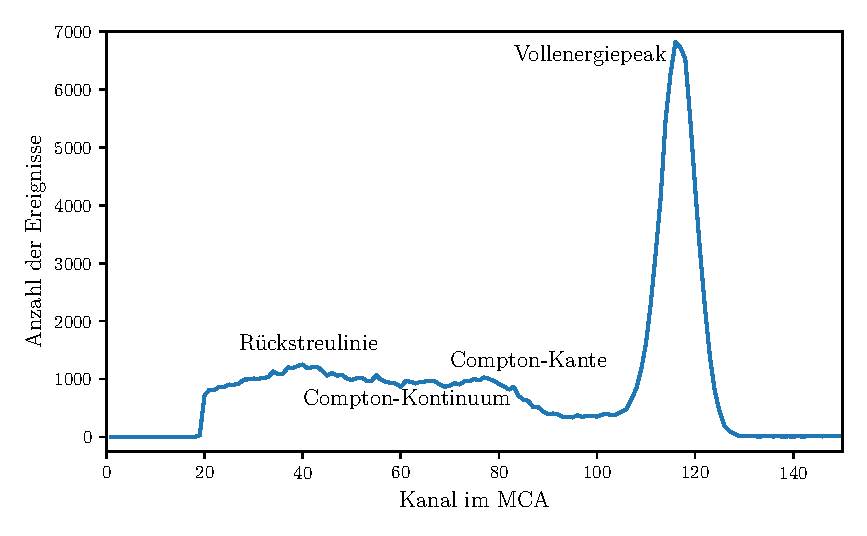
\includegraphics{spektrum.pdf}
    \caption{Das gemessene Spektrum der verwendeten Quelle. Dargestellt ist die Anzahl der Ereignisse \"uber den Kan\"alen des MCA.}
    \label{fig:spektrum}
\end{figure}

\subsection{Tomographie an homogenen W\"urfeln}

Zuerst wurde der leere W\"urfel aus Aluminium vermessen. Der Grund daf\"ur liegt in der Verwendung seiner abgeschw\"achten Intensit\"at als Eingangsintensit\"at f\"ur die Auswertung der anderen W\"urfel.
Die ermittelten Intensit\"aten f\"ur die Projektionen 2, 5 und 9 ergeben sich zu
\begin{align*}
  I_{P5} &= \SI{113.5(8)}{\becquerel}\\
  I_{P2} &= \SI{114.13(80)}{\becquerel}\\
  I_{P9} &= \SI{112.7(8)}{\becquerel}
\end{align*}

Als n\"achstes wird der zweite W\"urfel vermessen, welcher homogen aus einem Material besteht und von einer Aluminiumh\"ulle umschlo{\ss}en ist. Der Absorptionskoeffizient ergibt sich dabei 
\"uber folgende Gleichung:
\begin{align}
  \mu = \frac{1}{d}\cdot\symup{ln}\left(\frac{I_0}{I_i}\right),
\end{align}
mit der Ausgangsintensit\"at $I_2$ und $I_3$ des zweiten und dritten W\"urfels, sowie der Strecke $d$ die der Strahl je nach Projektion durchqueren muss. 
Diese Strecke betr\"agt f\"ur die zweite Projektion $3\sqrt{2}\symup{cm}$, f\"ur die f\"unfte Projektion $3\symup{cm}$ und f\"ur die
neunte Projektion $2\sqrt{2}\symup{cm}$. Als Wert f\"ur den Absorptionskoeffizienten wird der Mittelwert genommen.
Es ergibt sich ein Absorptionskoeffizienten des zweiten und dritten W\"urfels von
\begin{align*}
  \bar{\mu_2} &= \SI{0.568(3)}{\per\centi\metre}\\
  \bar{\mu_3} &= \SI{0.085(2)}{\per\centi\metre}\\
\end{align*}
Die gemessenen Counts und ermittelten Intensit\"aten f\"ur W\"urfel 2 und 3 sind in Tabelle \ref{tab:I23} aufgelistet.
In Tabelle \ref{tab:mu23} befinden sich die berechneten Absorptionskoeffizienten der einzelnen Projektionen.

\begin{table}%[htp]
  \centering
  \caption{Counts und Intensit\"aten f\"ur W\"urfel 2 und 3.}
  \label{tab:I23}
	\begin{tabular}{cccccc}
		  \toprule
			{$N_1$} & {$I_1$/(1/s)} & {$N_2$} & {$I_2$/(1/s)} & {$N_3$} & {$I_3$/(1/s)}\\
			\midrule
			\SI{34239(241)}{} & \SI{114.13(80)}{} & \SI{5794(98)}{}  & \SI{19.31(33)}{} & \SI{26690(208)}{} & \SI{88.97(69)}{}\\
			\SI{34058(239)}{} & \SI{113.53(80)}{} & \SI{3591(78)}{}  & \SI{11.97(26)}{} & \SI{23663(199)}{} & \SI{78.88(66)}{}\\
			\SI{33801(239)}{} & \SI{112.67(80)}{} & \SI{6528(103)}{} & \SI{21.76(34)}{} & \SI{26429(211)}{} & \SI{88.10(70)}{}\\
		  \bottomrule
	\end{tabular}
\end{table}

\begin{table}[htp]
	\begin{center}
  \caption{Ermitellte Absorptionskoeffizienten von W\"urfel 2 und 3.}
  \label{tab:mu23}
		\begin{tabular}{ccc}
		\toprule
			$\symup{Proj.}$ & $\mu_2/\SI{}{\per\centi\metre}$ & $\mu_3/\SI{}{\per\centi\metre}$\\
			\midrule
			5 & \SI{0.592(6)}{} & \SI{0.083(4)}{}\\
			2 & \SI{0.530(5)}{} & \SI{0.086(3)}{}\\
			9 & \SI{0.581(6)}{} & \SI{0.087(4)}{}\\
		\bottomrule
		\end{tabular}
	\end{center}
\end{table}

Ein Vergleich mit Theoriewerten~\cite{theorie} zeigt dass es sich beim zweiten W\"urfel um Eisen handelt, da der Theoriewert von $\SI{0.57}{\per\centi\metre}$ innerhalb des Fehlerintervalls liegt und damit keine Abweichung zeigt.
Der geringe Absorptionskoeffizient des dritten W\"urfels l\"asst auf ein leichtes Material wie Delrin schlie{\ss}en ($\mu_{\text{Delrin}}=\SI{0.11}{\per\centi\metre}$). Dies entspricht einer Abweichung
beim Delrin von $23\%$. 

\subsection{Tomographie am zusammengesetzten W\"urfel}

F\"ur den zusammengesetzten W\"urfel werden alle 12 Projektionen ausgewertet. Dies geschieht \"uber die Verwendung eines \"uberbestimmten Gleichungssystems, wie in Kapitel \ref{sec:Theorie} dargestellt.
Die 9 Elementarw\"urfel bestehen dabei jeweils aus dem Material des ersten oder zweiten homogenen W\"urfels.
Die gemessenen Counts und daraus ergebenden Intensit\"aten der 12 Projektionen sind in Tabelle \ref{tab:I5} aufgelistet. In Tabelle \ref{tab:mu5} befinden sich die ermittelten Absorptionskoeffizienten, sowie die jeweilige
vermutete Zuordnung des W\"urfels zu Eisen oder Delrin und dessen Theoriewerte~\cite{theorie} und Abweichungen.

\begin{table}[htp]
	\begin{center}
  \caption{Counts und Intensit\"aten des vierten W\"urfels.}
  \label{tab:I5}
		\begin{tabular}{cc}
		\toprule
			{$N_4$} & {$I_4$/(1/s)}\\
			\midrule
			\SI{13734(151)}{} & \SI{45.78(50)}{}\\
			\SI{11957(140)}{} & \SI{39.86(47)}{}\\
			\SI{12648(146)}{} & \SI{42.16(49)}{}\\
			\SI{5828(102)}{}  & \SI{19.43(34)}{}\\
			\SI{11528(138)}{} & \SI{38.43(46)}{}\\
			\SI{16669(167)}{} & \SI{55.56(56)}{}\\
			\SI{8713(121)}{}  & \SI{29.04(40)}{}\\
			\SI{6749(105)}{}  & \SI{22.50(35)}{}\\
			\SI{19400(180)}{} & \SI{64.67(60)}{}\\
			\SI{6572(106)}{}  & \SI{21.91(35)}{}\\
			\SI{16789(168)}{} & \SI{55.96(56)}{}\\
			\SI{15888(164)}{} & \SI{52.96(55)}{}\\
		\bottomrule
		\end{tabular}
	\end{center}
\end{table}

\begin{table}[htp]
	\begin{center}
  \caption{Vergleich zwischen den ermittelten Absorptionskoeffizienten und Theoriewerten.}
  \label{tab:mu5}
		\begin{tabular}{ccccc}
		\toprule
			$j$ & $\mu_2/\SI{}{\per\centi\metre}$ & $\text{Material}$ & $\mu_{\text{theorie}}$ & $\text{Abweichung}$\\
			\midrule
      1 &  \SI{0.464(9)}{}  & \text{Eisen}     & \SI{0.57}{}  &  18\%\\
      2 &  \SI{0.166(6)}{}  & \text{Delrin}    & \SI{0.11}{}  &  50\%\\
      3 & -\SI{0.020(8)}{}  & \text{Delrin}    & \SI{0.11}{}  &  118\%\\
      4 &  \SI{0.562(7)}{}  & \text{Eisen}     & \SI{0.57}{}  &  1\%\\
      5 &  \SI{0.132(7)}{}  & \text{Delrin}    & \SI{0.11}{}  &  20\%\\
      6 &  \SI{0.250(6)}{}  & \text{Delrin}    & \SI{0.11}{}  &  127\%\\
      7 &  \SI{0.664(10)}{} & \text{Eisen}     & \SI{0.57}{}  &  16\%\\
      8 &  \SI{0.420(7)}{}  & \text{Eisen}     & \SI{0.57}{}  &  26\%\\
      9 &  \SI{0.578(10)}{} & \text{Eisen}     & \SI{0.57}{}  &  1\%\\
      \bottomrule
		\end{tabular}
	\end{center}
\end{table}